\documentclass{standalone}

\usepackage{tikz}

\begin{document}


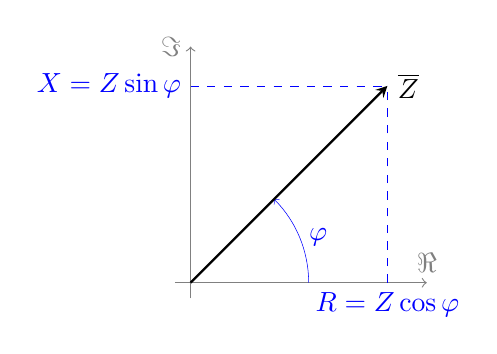
\begin{tikzpicture}
  \draw[->, thin, color=gray] (-0.2,0) -- (3,0) node[above] {$\Re$};
  \draw[->, thin, color=gray] (0,-0.2) -- (0,3) node[left] {$\Im$};
  \draw[-, very thin, dashed,color = blue] (2.5, 0) node[below] {$R = Z \cos\varphi$} -- (2.5, 2.5);
  \draw[-, very thin, dashed,color = blue] (0, 2.5) node[left] {$X = Z \sin\varphi$} -- (2.5, 2.5);
  \draw [->, very thin, color=blue](1.5,0)  arc[radius = 1.5, start angle= 0, end angle= 45] node [pos=0.5, right] {$\varphi$};
  \draw[->, >=stealth, thick, color = black] (0, 0) -- (2.5, 2.5) node[right] {$\overline{Z}$};

\end{tikzpicture}

\end{document}


